\section{Hardware}
\label{sec:Hardware}





\subsection{Sensoren}

Zur Messung der Drahtspannungskraft wird eine Wägezelle verwendet, mit Messbereich 0-1kg verwendet. Der Sensor besteht aus einem Metallblock mit zwei Bohrungen. Auf der ober und unter Seite des Blocks sind jeweils zwei Dehnmessstreifen einer 'Wheatstone Bridge' befestigt. Wird der Sensor durch Krafteinwirkung gebogen, so kann eine Spannungsänderung an den zwei abgegriffen Punkten $A^+$ und $A^-$ (siehe \autoref{fig:schaltplan}) eine Änderung der Spannung gemessen werden. Diese verhält sich im Messbereich annähernd linear. Durch Austesten konnte festgestellt werden, dass die Auflösung bei ca. 0.5~g liegt. Die Kalibrierung des Sensors wird in \autoref{sec:Messablauf} beschrieben.\newline
Ausgelesen wird der Sensor mittels eines 24-Bit-ADC´s am HX711-Board, von welchem die Daten danach über eine Serielleschnittstelle auf den Microcontroller und danach per USB an den Computer übertragen werden. Eine genauere Beschreibung der technischen Messumsetzung ist in \autoref{sec:Messschleife} ersichtlich. 


Weiters wurden zwei Endstopps verwendet. Diese sind einfache Taster welche ein Signal

% #TODO: schreiben
\subsection{Aktoren}

Als Aktoren wurden zwei ACT 24HS5430D8L2 NEMA23 Steppermotoren verwendet, da diese das für uns notwendige Haltemoment von 150~$N \cdot cm$ bieten. Das Funktionsprinzip eines Steppermotors ist die Ausrichtung eines Stators durch Erzeugung geeigneter Magnetfelder, mithilfe zweier Spulen. Der Aufbau des Motors ist auf der rechten Seite von \autoref{fig:schaltplan} ersichtlich. \newline
Zur Ansteuerung der Motoren wurden zwei TMC2209 Stepperdriver verwendet, welche zwar laut Datenblatt 2,5 A liefern können, von uns aus Gründen der Überhitzung nur bei ca. 1,7 A Belastung betrieben werden. Die vom Motor nutzbaren 3~$A~Phase^{-1}$ können somit noch nicht voll ausgeschöpft werden. Grund dafür ist eine Lieferverzögerung von aktuell ca. 2 Monaten der eigentlichen Treiber.


Die weiteren verwendeten Bauteile sind:
\begin{itemize}
    \item Arduino UNO (ATMEGA328p)
    \item Netzteil
    \item Stepdownconverter
\end{itemize}

\begin{figure}[H]
    \centering
    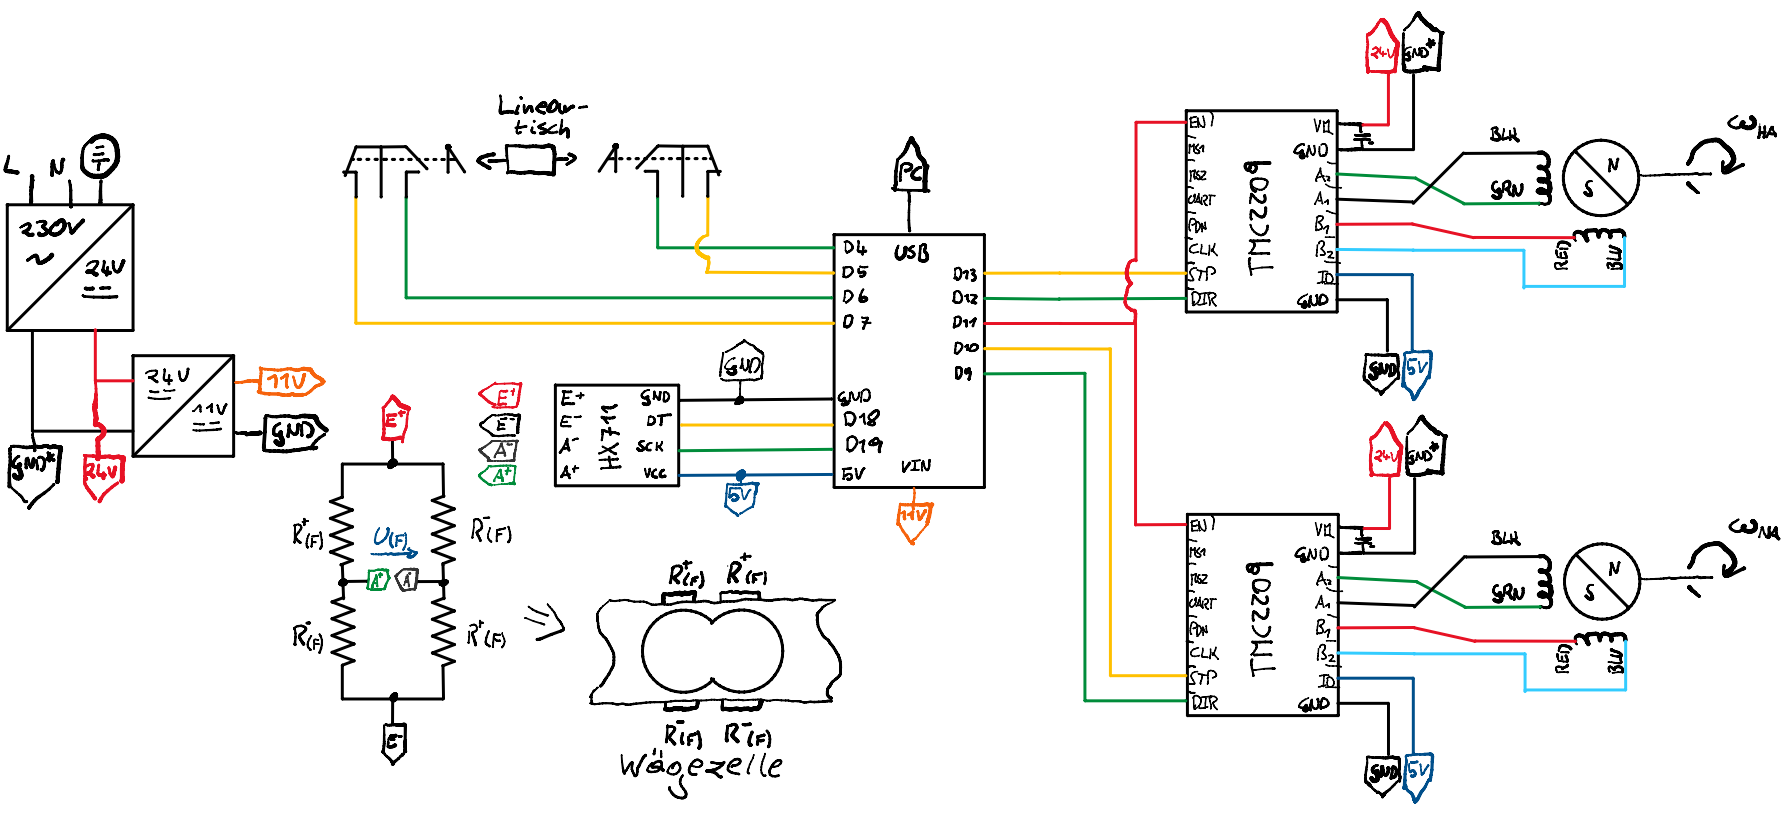
\includegraphics[width=1\textwidth]{./schaltplan.png}
    \caption{Schaltplan}
    \label{fig:schaltplan}
\end{figure}

In \autoref{fig:schaltplan} ist die elektronische Verschaltung des gesamten Projekt schematisch dargestellt. Der eingezeichnete Microcontroller, beschriftet mit 'USB', ist der Oben bereits erwähnte Arduino Uno. Die zwei, neben dem Lineartisch, eingezeichneten, und mit dem Microcontroller verschaltenen, Bauteile, sind die zwei Endstopps, welche im 'Normaly Open'-Modus $NO$ betrieben werden, um im Falle eines Kabelbruches einem Maschinenschaden vorzubeugen.